\documentclass[../main.tex]{subfiles}
\begin{document}

% \section{Kết luận}
Như vậy đồ án đã đạt được mục tiêu đề ra:
\begin{enumerate}
    \item Giải quyết bài toán sính số ngẫu nhiên trên mạng chuỗi khối.
    \item Đề xuất giải pháp giảm thiểu rủi ro, tăng tính phân tán trong mô hình sinh số ngẫu nhiên có thể kiểm chứng. 
\end{enumerate}
Ngoài ra, qua quá trình nghiên cứu và hoàn thành đồ án, em cũng rèn luyện thêm kỹ năng tìm kiếm, đọc tài liệu chuyên ngành; chọn lọc, tổng hợp kiến thức và chế bản đồ án bằng \LaTeX.

% \section{Hướng phát triển}
Trong giai đoạn phát triển tiếp theo, em đề xuất hai ý tưởng phát triển đồ án. 

Thứ nhất, DAO (Decentralized Autonomous Organization) sẽ là người chủ sở hữu của hợp đồng thông minh xác thực.

\begin{figure}[h!]
    \centering
    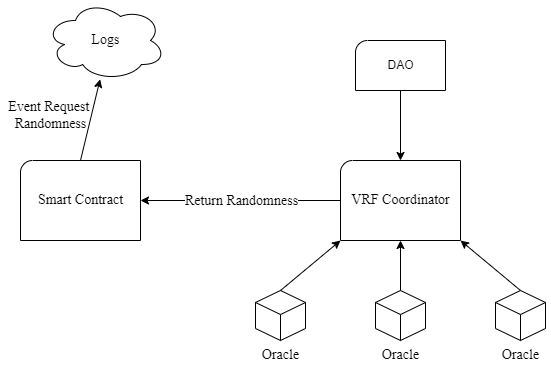
\includegraphics[scale = 0.5]{Figure/DAO.png}
    \caption{DAO tiếp quản hợp đồng thông minh VRF Coordinator}
    \label{fig:DAO}
\end{figure}

DAO giúp loại bỏ sự phụ thuộc vào một cá nhân hay tổ chức của hợp đồng xác thực. Dẫn ra cấu trúc kiểm soát phi tập trung từ việc trả thưởng cho các Oracle, trừng phạt các Oracle gian lận hay từ các tác vụ đơn giản như thêm Oracle được cung cấp dịch vụ... 

Thứ hai, sử dụng kỹ thuật ngưỡng chữ ký được trình bày trong \cite{stinson2001provably} để giảm thiểu chi phí tổng hợp các kết quả từ Oracle bằng cách đẩy việc này lên off-chain.

\begin{figure}[h!]
    \centering
    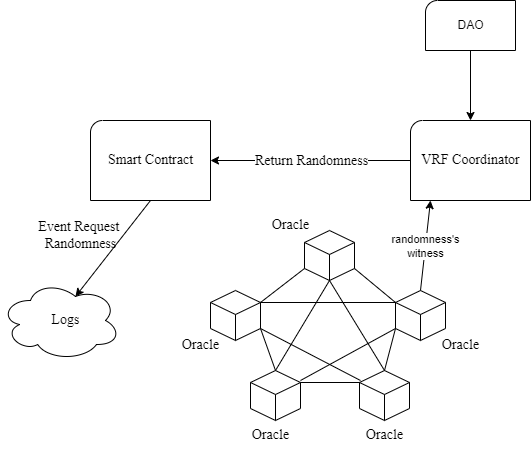
\includegraphics[scale = 0.6]{Figure/thresholdSignature.png}
    \caption{Mô hình sinh số ngẫu nhiên sử dụng mạng lưới các Oracle}
    \label{fig:thresholdSignature}
\end{figure}

Trong mô hình được trình bày ở hình \ref{fig:thresholdSignature}, mỗi Oracle đóng vai trò như là một node trong mạng lưới. Xác thực và tổng hợp các kết quả ngẫu nhiên trên từng node và gửi kết quả cuối cùng với chữ ký ngưỡng sẽ giảm được chi phí xác thực bằng chứng ngẫu nhiên nhiều lần với mỗi yêu cầu của hợp đồng khách hàng, mà vẫn đảm bảo được tính trung thực của các Oracle.
\end{document}
